\documentclass[conference]{IEEEtran}
\IEEEoverridecommandlockouts
% The preceding line is only needed to identify funding in the first footnote. If that is unneeded, please comment it out.
\usepackage{cite}
\usepackage{amsmath,amssymb,amsfonts}
\usepackage{algorithmic}
\usepackage{graphicx}
\usepackage{textcomp}
\usepackage{xcolor}
\usepackage{hyperref}
\usepackage[colorinlistoftodos]{todonotes}
\usepackage[xindy]{glossaries} 
\usepackage[utf8]{inputenc}
\pagenumbering{arabic}
\newacronym{pca}{PCA}{Principal Component Analysis}
\newacronym{svc}{SVC}{C-Support Vector Classification}
\newacronym{dtc}{DTC}{Decision Tree Classifier}
\newacronym{lr}{LR}{Logistic Regression}
\newacronym{gnb}{GNB}{Gaussian NB}
\newacronym{lda}{LDA}{Linear Discriminant Analysis}
\newacronym{cnn}{CNN}{Convolutional Neural Network}
\newacronym{kfcv}{K-FCV}{K-Fold Cross Validation}
\newacronym{loocv}{LOOCV}{Leave-One-Out Cross Validation}
\makeglossaries


\def\BibTeX{{\rm B\kern-.05em{\sc i\kern-.025em b}\kern-.08em
    T\kern-.1667em\lower.7ex\hbox{E}\kern-.125emX}}
\graphicspath{ {./images/} }
\begin{document}


\title{Face Recognition with Olivetti dataset\\}

\author{\IEEEauthorblockN{Lucius Filho 96123}
\IEEEauthorblockA{\textit{DETI} \\
\textit{University of Aveiro}\\
Aveiro, Portugal\\
luciusviniciusf@ua.pt}
\and
\IEEEauthorblockN{Tomé Carvalho 97939}
\IEEEauthorblockA{\textit{DETI} \\
\textit{University of Aveiro}\\
Aveiro, Portugal \\
tomecarvalho@ua.pt}
}

\maketitle
\thispagestyle{plain}
\pagestyle{plain}


\begin{abstract}
The Olivetti dataset was chosen from the proposal list in the project instructions, available on Kaggle. \cite{olivetti_dataset}. Facial recognition is a technology capable of matching a human face from a digital image or a video frame against a database of faces in order to identify the person.
Our main goal in this project is to explore different machine learning models that can be used in such a system and compare their performance.
\end{abstract}

\begin{IEEEkeywords}
facial recognition, machine learning, classification, data analysis, logistic, c-support vector classification, linear discriminant analysis, gaussian naive bayes, k neighbors, decision tree, convolutional neural network, deep learning, principal component analysis
\end{IEEEkeywords}

\section{Introduction}
Nowadays, facial recognition is ubiquitous in our day-to-day life. It has various different applications\cite{trio}.

The most well-known application is likely security and surveillance. Governments, businesses and other entities can use it to identify criminal suspects.

Another common use is for biometric authentication. The most intuitive example is unlocking smartphones, using technologies such as Android's Face Unlock or Apple's Face ID.

Additionally, it is also used for purposes such as assisting in the search for missing people, facial reconstruction (e.g., of witnesses), etc.

As it is quite a relevant technology with a multitude of different applications, it is useful to investigate which models lead to robust implementations, our objective in this project.

\section{State-of-the-art Review}

Paper\cite{clarifai_paper} states that CNN have been found to be the most useful and accurate type of deep learning method for face recognition, the benefit of using neural networks is that it can reduce the dimensionality and can be trained as a classifier and that the most common architectures used for CNN are VGGnet and GoogleNet, both achieving a very comparable level of face recognition accuracy.

Paper\cite{modi_patel_paper} highlights six types of algorithms: SVM, CNN, Eigenface based algorithms, Gabor Wavelet, PCA, and HMM. It referenced other papers, comparing the performance results of each type of algorithm across them, although the results seemed to vary a significant amount.

\begin{figure}[]
    \centering
    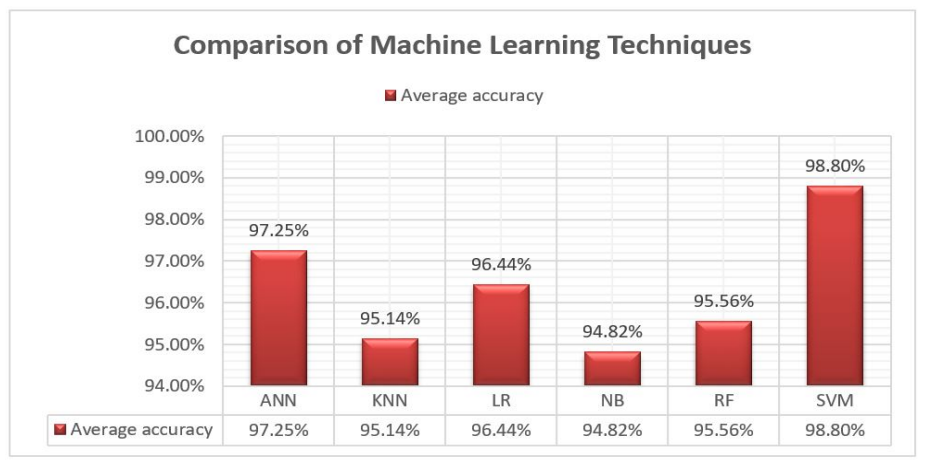
\includegraphics[scale=0.45]{images/12_hal_comparison.png}
    \caption{Comparison of Machine Learning Techniques\cite{hal_paper}}
    \label{fig:hal_comparison}
\end{figure}

Fig. \ref{fig:hal_comparison}, from paper\cite{hal_paper} compares the accuracy of multiple traditional (non-deep learning) machine learning methods. Support Vector Machines (SVM) showed the best results, 98.80\%, followed by Artificial Neural Networks with 97.25\% (ANN) and Logistic Regression (LR) with 96.44\%. K-nearest Neighbors (KNN), Naive Bayes (NB) and Random Forest (RF) paled in comparison to these, with 95.14\%, 94.82\% and 95.56\% accuracy, respectively.



\begin{figure}[]
    \centering
    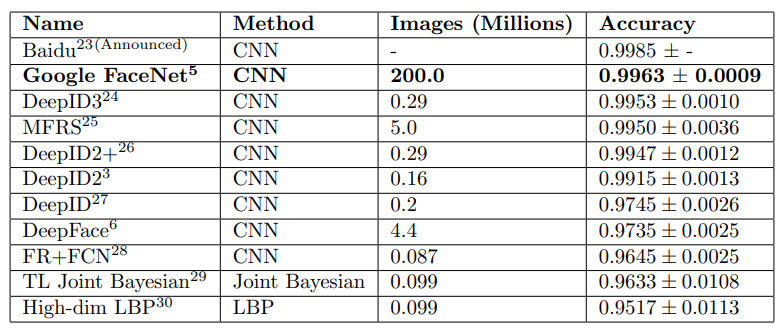
\includegraphics[scale=0.5]{images/13_balaban_table.png}
    \caption{Comparison of Facial Recognition Systems\cite{hal_paper}}
    \label{fig:balaban_table}
\end{figure}

Fig. \ref{fig:balaban_table}, from paper\cite{balaban_paper} compares the accuracy of eleven state-of-the-art facial recognition systems, highlighting Google FaceNet, with an outstanding accuracy of 99.63\% as the winner. Out of the systems listed, nine use Convolutional Neural Network (CNN) as the machine learning model. This was a great incentive for us to apply the CNN deep learning model to our dataset.

\begin{figure}[]
    \centering
    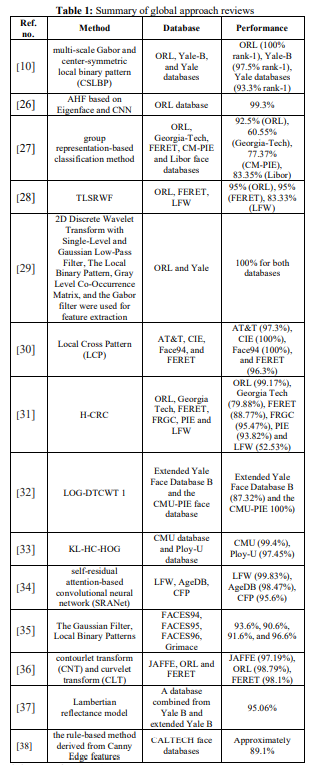
\includegraphics[scale=1]{images/14_moung_table.png}
    \caption{Summary of global approach reviews\cite{moung_paper}}
    \label{fig:moung_table}
\end{figure}


Fig. \ref{fig:moung_table}, from paper\cite{moung_paper} compares specific methods' performance across several databases. The vast majority of them are out of the scope of the subject. Nevertheless, CNN is mentioned again in the second approach, which had an accuracy of 99.3\% on the ORL database, further incentivizing us to implement CNN.

\section{Dataset}

\subsection{Dataset description}

The dataset used is available on Kaggle \cite{olivetti_dataset}. Credits to AT\&T Laboratories Cambridge\cite{att_labs_cambridge}.
It comprises a total of 400 face images, with the following properties:
\begin{itemize}
\item Images taken between April 1992 and April 1994 at AT\&T Laboratories Cambridge.
\item There are ten different images of each of the 40 distinct people.
\item The images were taken at different times with variations of lighting, facial expressions and facial details.
\item The background of the images is black.
\item The images are grayscale.
\item The dimension of each image is 64x64 pixels.
\item Image pixel values were scaled down to the [0, 1] interval.
\item The names of the 40 people were encoded to integer IDs, from 0 to 39.
\end{itemize}

\subsection{Preprocessing}

As previously stated, the images are grayscale, and, in addition, their pixels' values have already been downscaled to values in [0, 1]. That being the case, it was not necessary to apply normalization.

It is, however, worth nothing that we had to reshape the training and test X data to (-1, 64, 64, 1) so that it would be compatible with the 2D convolution layers' input shape.

\begin{figure}[]
    \centering
    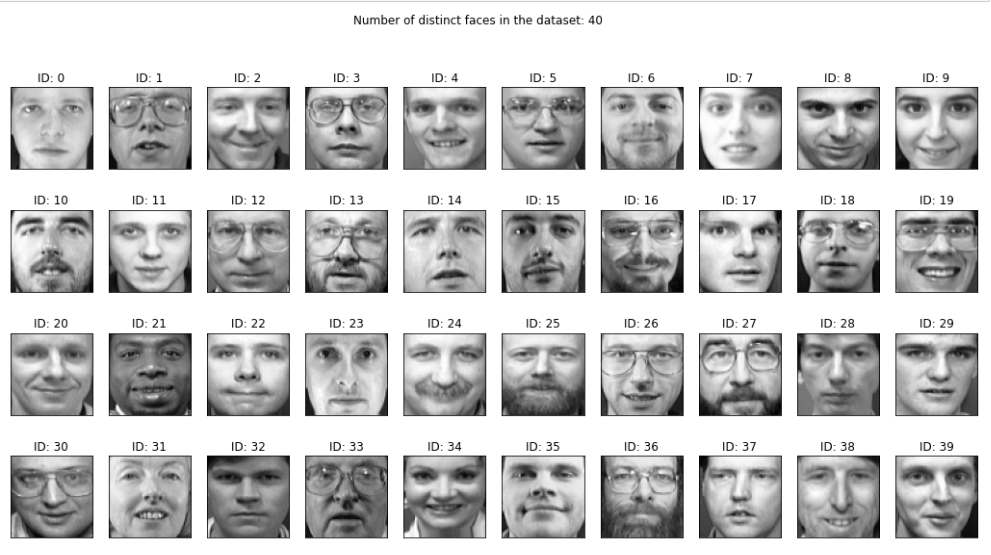
\includegraphics[scale=0.4]{images/0_distinct_faces.png}
    \caption{An image from each distinct individual in the dataset.}
    \label{fig:distinct_faces}
\end{figure}

\subsection{Feature distribution}

\begin{figure}[]
    \centering
    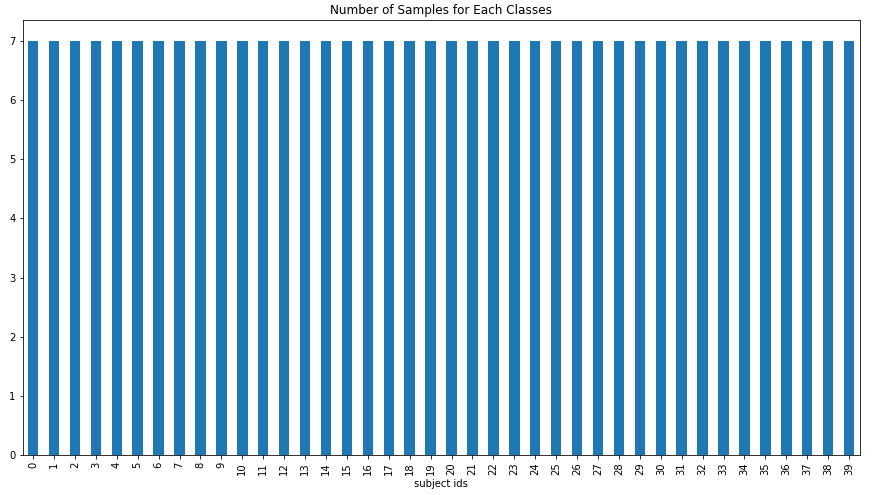
\includegraphics[scale=0.45]{images/2_samples_per_class.png}
    \caption{Distribution of images for each person.}
    \label{fig:samples_per_class}
\end{figure}

Fig. \ref{fig:samples_per_class} confirms that the dataset's 400 images are distributed among 40 different people, with 10 images for each one. 

\begin{figure}[]
    \centering
    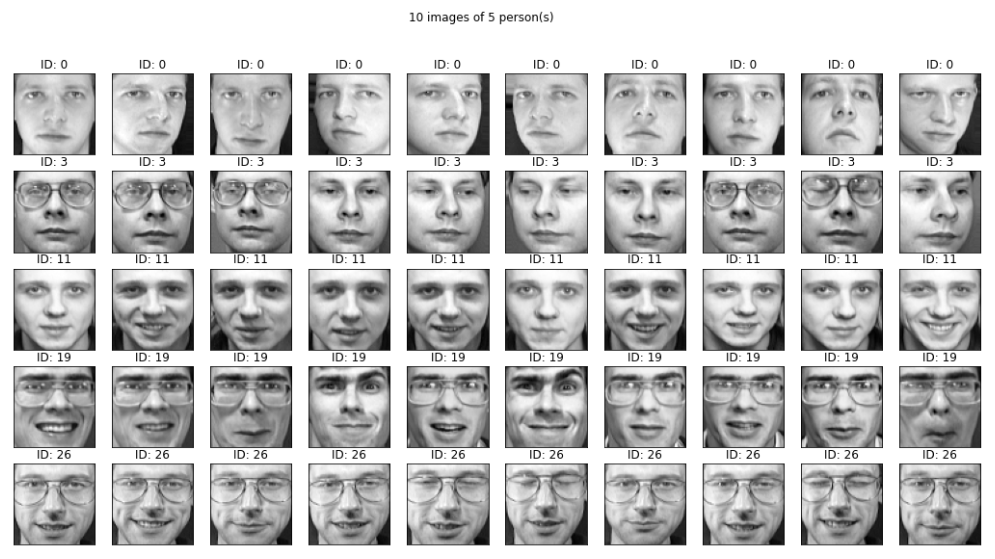
\includegraphics[scale=0.4]{images/1_imgs_of_persons.png}
    \caption{Group of face images for each person.}
    \label{fig:imgs_of_persons}
\end{figure}

Fig. \ref{fig:imgs_of_persons} shows the 10 images of 5 randomly selected subjects from the dataset.



According with Fig. \ref{fig:lda_confusion_matrix}, its possible to see that, using LDA, most faces are correctly categorized frequently. However, there are a few exceptions which were more often confused.

\subsection{Principal Component Analysis}

\gls{pca} was used for dimensionality reduction. In order to make an appropriate choice of the number of components, we made use of a convenient property of scikit-learn's PCA object's \textit{n\_components} parameter: passing a number in ]0, 1[ will select the minimum number of components such that the explained variance is greater than the percentage specified by \textit{n\_components}. We experimented setting the desired retained variance to values between 90\% and 99\%, with steps of 1\%. We had also experimented with 0.89 earlier on, but our observations were not relevant. That is the reason why LOO cross-validation does not have data for this value of the desired retained variance. We found 90\% to be the value that yielded the best results. As evidenced in Figs. \ref{fig:variances} and \ref{fig:variances-log}, the corresponding number of components \textit{k} was 66.

\begin{figure}
    \centering
    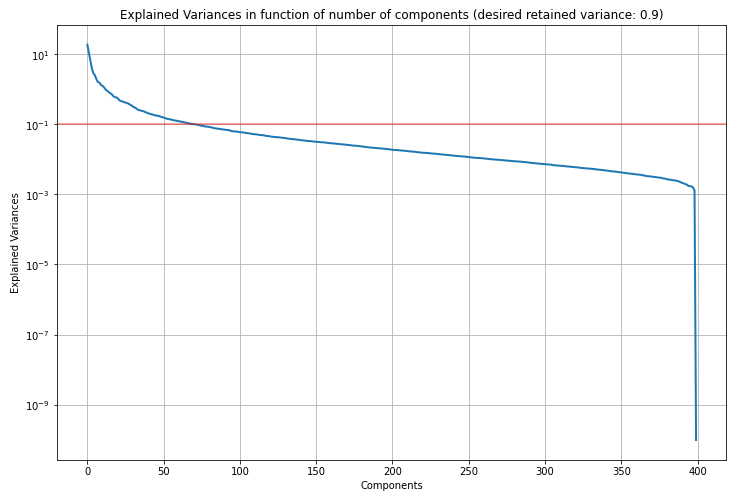
\includegraphics[scale=0.5]{images/4_explained_vars.png}
    \caption{Explained Variances in function of number of components.}
    \label{fig:variances}
\end{figure}

\begin{figure}
    \centering
    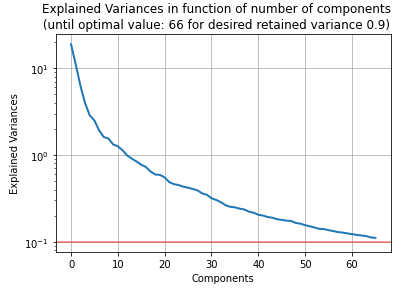
\includegraphics[scale=1]{images/5_explained_vars_until_k.png}
    \caption{Explained Variances in function of number of components with logarithm scale.}
    \label{fig:variances-log}
\end{figure}

\begin{figure}
    \centering
    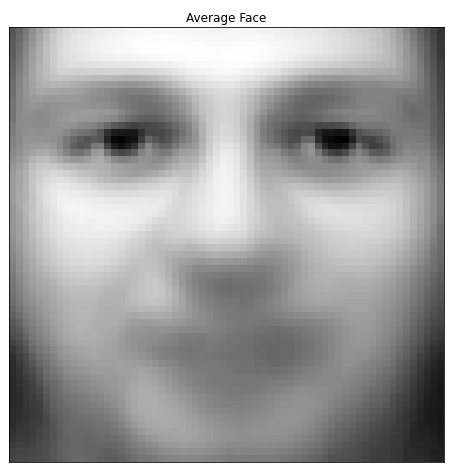
\includegraphics[scale=0.75]{images/6_average_face.png}
    \caption{Average Face determined by the \gls{pca}.}
    \label{fig:average_face}
\end{figure}

The average face resulting from PCA is visible in Fig. \ref{fig:average_face}.

\begin{figure}
    \centering
    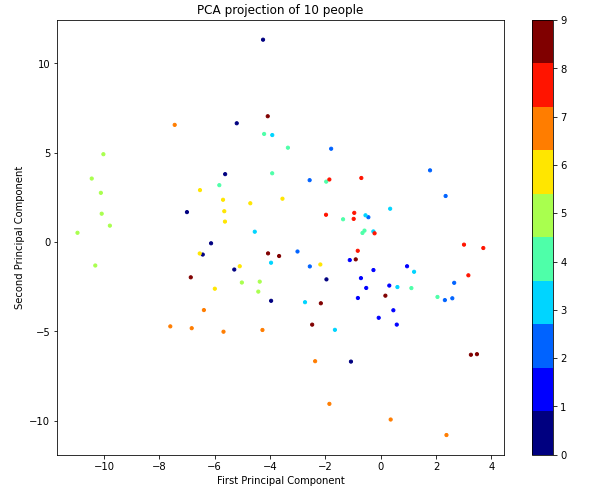
\includegraphics[scale=0.75]{images/3_pca_projection_10_people.png}
    \caption{PCA: Projection of the first two components of 10 people.}
    \label{fig:pca_projection_10_people}
\end{figure}

Fig. \ref{fig:pca_projection_10_people} plots the first two principal components of ten people from the dataset. The most notable example is seen in the left side of the graph,  where a lot of the fifth person's images are found close together. We must keep in mind that this visualization encompasses only the first two principal components, which is only 3\% of the number of components kept.

\begin{figure}
    \centering
    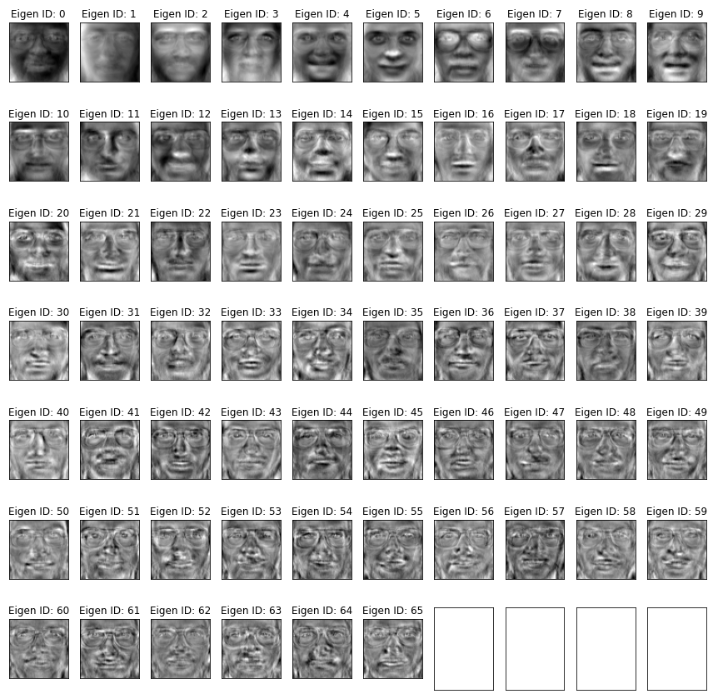
\includegraphics[scale=0.5]{images/7_eigenfaces.png}
    \caption{Eigenfaces}
    \label{fig:eigenfaces}
\end{figure}

Each PCA component corresponds to an eigenface, which is the graphical representation of an eigenvector. Eigenfaces are a useful method for facial recognition and detection, by determining the variance of faces in a collection of face images and using those variances to encode and decode a face in a machine learning way without the full information, reducing computation and space complexity. All 66 eigenfaces are displayed, in the corresponding PCA component order, in Fig. \ref{fig:eigenfaces}.


\section{Regression Model}

\subsection{Types of regression}

Since the goal is to identify the face's person, the use of a classification model is necessary. We applied the following classification methods:

\begin{itemize}
  \item \textbf{\gls{lda}}\cite{linear_reg}: fits a Gaussian density to each class, assuming that all classes share the same covariance matrix.
  \item \textbf{\gls{lr}} \cite{random_forest_reg}: predicts a dependent data variable by analyzing the relationship between one or more existing independent variables.
  \item \textbf{\gls{gnb}} \cite{gaussian_nb}:  performs online updates to model parameters via $partial_fit$.
  \item \textbf{\gls{dtc}} \cite{decision_tree}: has the capability of capturing descriptive decision making knowledge from the supplied data.
  \item \textbf{\gls{svc}} \cite{svc_sklearn}: implements LIBSVM\cite{libsvm}, which implements linear SVMs and logistic regression models trained using a coordinate descent algorithm.
  \item \textbf{\gls{cnn}} \cite{cnn}: a neural network, in this particular case, with 11 layers, including 2D convolution , 2D max pooling, dropout, flatten, and dense layers.
\end{itemize}



\subsection{Testing accuracy}

To obtain the most accurate model, we proceeded to analyze the accuracy of each aforementioned model using the following methods:

\begin{itemize}
    \item \textbf{Simple Validation}: Distribution of the Train and Test samples (7:3 ratio). The model then fits the training samples and evaluate the test. In Fig. \ref{fig:simple-validation} shows the accuracies obtained with this method.
    \item \textbf{\gls{kfcv}}: Distributes all samples between Train and Test groups (folds) multiple times. Fig. \ref{fig:k-fold-accuracy} represents its accuracy.
    \item \textbf{\gls{loocv}}: Because \gls{kfcv} is fold-based and the dataset does not have a lot of data, but only 400 images, \gls{loocv} was used as a better alternative to \gls{kfcv}. The former uses a similar strategy, but instead of splitting the data into K folds, each sample is used once as a test set (singleton) while the remaining samples form the training set. Its results are shown in Fig. \ref{fig:leave-one}.
    \item \textbf{Deep Learning}: CNN, being a deep learning method, had to be handled separately. Unlike the basis we used\cite{olivetti_knn_cnn}, we did not use a generator and \textit{fit\_generator}, using \textit{fit} instead and then plotting the accuracy and loss over the epochs.
\end{itemize}

\subsection{Graphical representation of results}

\begin{figure}
    \centering
    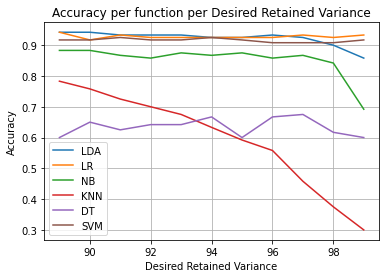
\includegraphics[scale=0.65]{images/15_Accuracy_per_function_per_Desired_Retained_Variance.png}
    \caption{Accuracy of each classifier in the Simple Validation method.}
    \label{fig:simple-validation}
\end{figure}

\begin{figure}
    \centering
    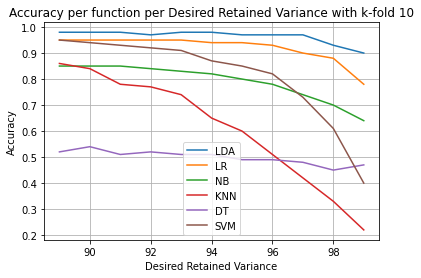
\includegraphics[scale=0.58]{images/16_Accuracy_per_function_per_Desired_Retained_Variance_with_k-fold_10.png}
    \caption{Accuracy of each classifier in the \gls{kfcv} method.}
    \label{fig:k-fold-accuracy}
\end{figure}

\begin{figure}
    \centering
    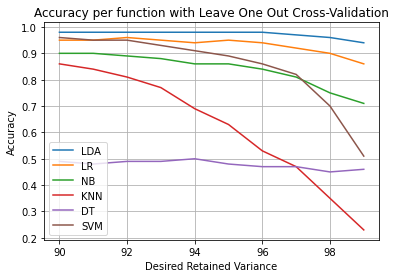
\includegraphics[scale=0.6]{images/17_Accuracy_per_function_with_Leave_One_Out_Cross-Validation.png}
    \caption{Accuracy of each classifier in the \gls{loocv} method.}
    \label{fig:leave-one}
\end{figure}

\begin{figure}
    \centering
    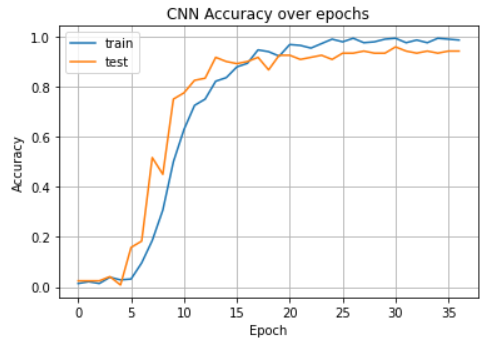
\includegraphics[scale=0.75]{images/10_cnn_accuracy.png}
    \caption{\gls{cnn}'s accuracy in the Deep Learning method.}
    \label{fig:deep-learning-accuracy}
\end{figure}

\begin{figure}
    \centering
    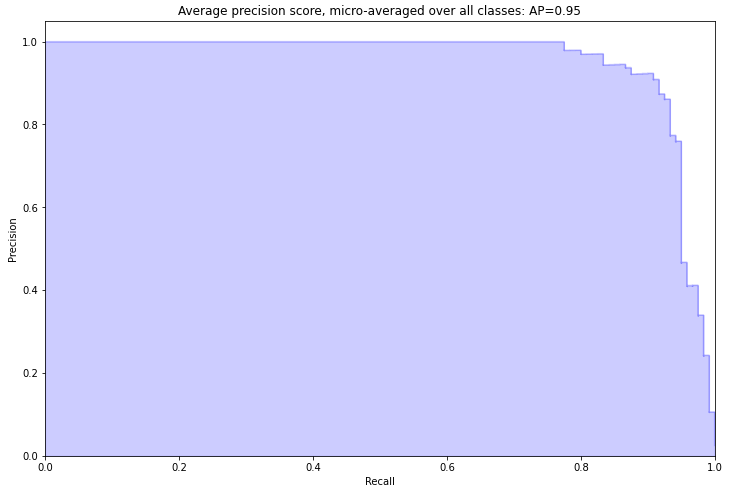
\includegraphics[scale=0.5]{images/9_precision_recall_roc_curves.png}
    \caption{LDA Precision Recall Curve}
    \label{fig:precision_recall_roc_curves}
\end{figure}


\begin{table}
\caption{Maximum Accuracy By Each Method}
\begin{center}
\begin{tabular}{|c|c|c|}
\hline
\textbf{Method} & \textbf{Best Classifier} & \textbf{Max. Accuracy} \\
\cline{1-2} 
\hline
Simple Validation & \gls{lda} & 0.942 \\
\hline
\gls{kfcv} & \gls{lda} & 0.980 \\
\hline
\gls{loocv} & \gls{lda} & 0.980  \\
\hline
Deep Learning & \gls{cnn} & 0.985\\

\hline
\end{tabular}
\label{methods-table}
\end{center}
\end{table}

Observing Table \ref{methods-table} along with Figs. \ref{fig:simple-validation}, \ref{fig:k-fold-accuracy}, \ref{fig:leave-one} and \ref{fig:deep-learning-accuracy}, it is possible to conclude that LDA was the best performing method among the traditional ones, while CNN, the deep learning method, was able to perform slightly better.

\subsubsection{Linear Discriminant Analysis Confusion Matrix}
Since \gls{lda} proved to perform the best out of the traditional machine learning models, we found it relevant to plot its confusion matrix at Fig. \ref{fig:lda_confusion_matrix}. Additionally, Fig. \ref{fig:precision_recall_roc_curves}, shows that LDA was able to achieve both good accuracy and precision values.

\begin{figure}[]
    \centering
    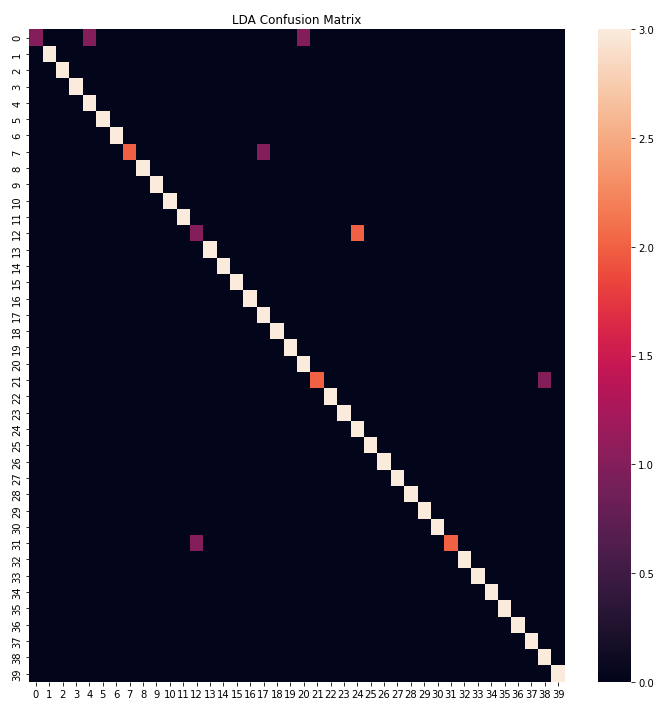
\includegraphics[scale=0.5]{images/8_lda_confusion_matrix.png}
    \caption{\gls{lda} Confusion Matrix.}
    \label{fig:lda_confusion_matrix}
\end{figure}

\subsection{Feature Importances in the Random Forest Regression}

\section{Conclusion}
Regarding our results, LDA had the best accuracy among the traditional machine learning methods, for all validation strategies (simple validation 94.2\%, K-fold cross-validation and leave-one-out cross-validation 98\%).
The deep learning method, CNN, achieved a slightly higher accuracy of 98.5\%.

We were able to accomplish the goals of our project successfully. Namely, investigating state-of-the-art facial recognition methods, analyzing the dataset, applying and comparing multiple methods of classification, including a deep learning one, as well as drawing conclusions from the results obtained.

\section{Division of labor}
Both students collaborated an equal amount through online meetings for synchronous development, in order to achieve collective responsibility over the entirety of the project.

\glsaddall
\printglossary
\addcontentsline{toc}{section}{Glossary}


\begin{thebibliography}{00}

\bibitem{olivetti_dataset}
\href{https://www.kaggle.com/datasets/imrandude/olivetti}{Olivetti Dataset}

\bibitem{att_labs_cambridge}
\href{https://cam-orl.co.uk/index.html}{AT\&T Laboratories Cambridge}

\bibitem{trio}
\href{https://www.trio.dev/blog/facial-recognition-applications}{Trio: Facial Recognition Applications}

\bibitem{hal_paper}
\href{https://hal.inria.fr/hal-03620410/document}{Comparative study of machine learning algorithms for
face recognition}

\bibitem{clarifai_paper}
\href{https://www.clarifai.com/hubfs/Ebooks/whitepaper-machine-learning-approaches-face-detection.pdf}{Machine learning approaches to face detection
and recognition}

\bibitem{balaban_paper}
\href{https://arxiv.org/pdf/1902.03524.pdf}{Deep learning and face recognition: the state of the art}

\bibitem{modi_patel_paper}
\href{https://www.igi-global.com/pdf.aspx?tid=283961&ptid=278106&ctid=4&oa=true&isxn=9781683182122}{A State-of-the-Art Survey on Face Recognition Methods}

\bibitem{moung_paper}
\href{https://www.warse.org/IJATCSE/static/pdf/file/ijatcse16912sl2020.pdf}{Face Recognition State-of-the-art, Enablers, Challenges and Solutions: Review}

\bibitem{olivetti_knn_cnn}
\href{https://www.kaggle.com/code/tareksherif/olivetti-classification-useing-knn-cnn-for-fun/notebook}{Olivetti Classification using KNN and CNN}

\bibitem{linear_reg} 
\href{https://scikit-learn.org/stable/modules/generated/sklearn.discriminant_analysis.LinearDiscriminantAnalysis.html}{Sklearn - Linear Discriminant Analysis}

\bibitem{random_forest_reg}
\href{https://scikit-learn.org/stable/modules/generated/sklearn.ensemble.RandomForestRegressor.html}{Sklearn - Random Forest Regressor}

\bibitem{logistc_reg}
\href{https://www.techtarget.com/searchbusinessanalytics/definition/logistic-regression#:~:text=Logistic\%20regression\%20is\%20a\%20statistical,or\%20more\%20existing\%20independent\%20variables.}{What is Logistic Regression - Tech Target}

\bibitem{gaussian_nb}
\href{https://scikit-learn.org/stable/modules/generated/sklearn.naive_bayes.GaussianNB.html}{Sklearn - GaussianNB}

\bibitem{decision_tree}
\href{https://www.sciencedirect.com/topics/computer-science/decision-tree-classifier}{Decision Tree Classifier - an overview - ScienceDirect Topics}

\bibitem{svc_sklearn}
\href{https://scikit-learn.org/stable/modules/generated/sklearn.svm.SVC.html}{Sklearn - SVC}

\bibitem{libsvm}
\href{https://en.wikipedia.org/wiki/LIBSVM}{LIBSVM - Wikipedia}

\bibitem{cnn}
\href{https://en.wikipedia.org/wiki/Convolutional_neural_network}{CNN - Wikipedia}
\end{thebibliography}

\end{document}